\documentclass[fleqn]{article}
\oddsidemargin 0.0in
\textwidth 6.0in
\thispagestyle{empty}
\usepackage{import}
\usepackage{amsmath}
\usepackage{amsfonts}
\usepackage{bigints}
\usepackage{graphicx}
\usepackage[english]{babel}
\usepackage[utf8x]{inputenc}
\usepackage{float}
\usepackage[colorinlistoftodos]{todonotes}

\definecolor{hwColor}{HTML}{AD53BA}

\begin{document}

  \begin{titlepage}

    \newcommand{\HRule}{\rule{\linewidth}{0.5mm}} % Defines a new command for the horizontal lines, change thickness here

    \center % Center everything on the page


    \textsc{\LARGE Arizona State University}\\[1.5cm] % Name of your university/college

    \textsc{\LARGE Mathematical Methods For Physics I }\\[1.5cm] % Major heading such as course name


    \begin{figure}
      
\includegraphics[width=\linewidth]{asu.png}
    \end{figure}


    \HRule \\[0.4cm]
    { \huge \bfseries Homework 15}\\[0.4cm] 
    \HRule \\[1.5cm]

    \textbf{Behnam Amiri}

    \bigbreak

    \textbf{Prof: Cecilia Lunardini}

    \bigbreak


    \textbf{{\large \today}\\[2cm]}

    \vfill % Fill the rest of the page with whitespace

  \end{titlepage}

  \begin{enumerate}
  \item  (Note: this part was assigned in homework 14 as a bonus. If you have done it then (fully and completely), you are not required to repeat it. ): 

    \begin{enumerate}
    \item Set up separation constants, discuss their signs, and write the general solution for the wave equation (Hint: how many \emph{independent} separation constants do we have here?).

      \textcolor{hwColor}{
        We seek to solve the following: \\
      }

      \begin{figure}[htbp] 
        \begin{center} 
          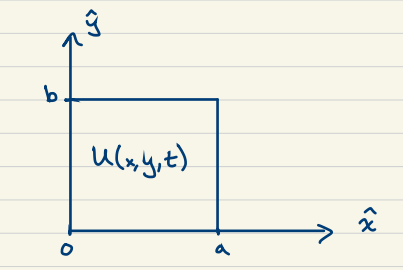
\includegraphics[height=4cm, width=7cm]{drum.PNG} 
        \label{default} 
        \end{center} 
      \end{figure} 

      \textcolor{hwColor}{
        We are required to solve the following 2-D wave equation: \\
        $
          \bigtriangledown^2 u=\dfrac{1}{v^2}\dfrac{\partial^2 u}{\partial t^2} \\
        $
      }

      \textcolor{hwColor}{
        We begin by assuming that equation is of a separable form (Otherwise what the heck are we doing here?), thus we assume a solution of the following form. \\
        \\
        $u(x,y,t)=X(x)Y(y)T(t)$ \\
        \\
        Where all functions on the RHS are there of only respective varibales. Plugging this back into our differential equation gives: \\
        \\
        $
          \bigtriangledown^2 u=\dfrac{1}{v^2}\dfrac{\partial^2 u}{\partial t^2} \\
          \\
          \dfrac{\partial^2 u}{\partial x^2}+\dfrac{\partial^2 u}{\partial y^2}=\dfrac{1}{v^2}\dfrac{\partial^2 u}{\partial t^2} \\
          \\
          X^{''}(x)Y(y)T(t)+X(x)Y^{''}(y)T(t)=\dfrac{1}{v^2}X(x)Y(y)T^{''}(t) \\
          \\
        $
        Where here we allow $X^{''}(x)=\dfrac{\partial^2 X}{\partial x}$, for example. \\
        Now dividing both sides of the equation by $u(x,y,t)$ we get: \\
        \\
        $
          \dfrac{X^{''}}{X}+\dfrac{Y^{''}}{Y}=\dfrac{1}{v^2}\dfrac{T^{''}}{T} \\
          \\
        $
        This is the equation we will be evaluating.
      }

      \textcolor{hwColor}{
        \underline{Important}: We now note, since each function in the above equation is a function of \textbf{\textit{only}} its respective varaible,
        that the \underline{only way} the above can be true is when both sides are equal to the same constant. Thus, \\
        \\
        $
          \dfrac{X^{''}}{X}+\dfrac{Y^{''}}{Y}=\dfrac{1}{v^2}\dfrac{T^{''}}{T}=\mu \\
          \\
        $
        With $\mu$ constant. This leaves us with the following systme f equations. \\
        \\
        $
          \begin{cases}
            T^{''}-\mu v^2 T=0 ~~~~~~~ (1) \\
            \dfrac{X^{''}}{X}=-\dfrac{Y^{''}}{Y}+\mu ~~~~~ (2)
          \end{cases} \\
          \\
        $
        Again, we note (2) is only true when both sides are equal to a constant. Thus, \\
        \\
        $
          \dfrac{X^{''}}{X}=\gamma=-\dfrac{Y^{''}}{Y}+\mu \\
          \\
        $
        Such that \\
        \\
        $
          X^{''}-\gamma X=0 \\
          Y^{''}-(\mu-\gamma)Y=0 \\
          \\
        $
        If we let $\sigma=\mu-\gamma$, then then second equation above can be rewritten: \\
        \\
        $
          Y^{''}-\sigma Y=0
        $ \\
        So now we are left with the following system of equations. \\
        \\
        $
          \begin{cases}
            T^{''}-\mu v^2 T=0 \\
            X^{''}- \gamma X=0 \\
            Y^{''}-\sigma Y=0
          \end{cases}
        $ \\
        With $\mu ~~ \gamma ~~ \sigma$ related by: $\sigma=\mu-\gamma$ \\
      }

      \textcolor{hwColor}{ 
        \rule{16cm}{1pt} 
      }

      \textcolor{hwColor}{
        Now let us consider one of the above equations, for example. $X^{''}-\gamma X=0$ \\
        \\
        We examine the three possilbe cases for constant $\gamma$, namely $\gamma >0 ~~~ \gamma=0 ~~~ ,and ~~~ \gamma <0$ \\
        \\
        Let $\gamma=\alpha^2$, then for $\gamma > 0$, we have $\rightarrow X^{''}-\alpha^2 X=0 ~~~~ (3)$ \\
        \\
        Where we will assume the following solution: \\
        $
          \begin{cases}
            X(x)=Ae^{\alpha x}+B e^{-\alpha x} \\
            \\
            X^{'}(x)=\alpha Ae^{\alpha x}- \alpha B e^{-\alpha x} \\
            \\
            X^{''}(x)=\alpha^2 Ae^{\alpha x}+\alpha^2 Be^{-\alpha x}
          \end{cases} \\
        $
        \\
        This is where we can see this satisfies (3).
      }

      \textcolor{hwColor}{
        For $\gamma=0$, we have $X^{''}-(0)X=0 \longrightarrow X^{''}=0$ \\
        \\
        This we will denote the \underline{trivial solution} and discard for now. \\
        \\
      }

      \textcolor{hwColor}{ 
        \rule{16cm}{1pt} 
      }

      \textcolor{hwColor}{
        For $\gamma<0$, we have \\
        $
          X^{''}+\alpha^2 X=0 ~~~~ (4) \\
          \\
        $
        Where we will assume a solution of the following form: \\
        \\
        $X(x)=Ccos(\alpha x)+Dsin(\alpha x)$ \\
        \\
        Thus,\\
        \\
        $
          \begin{cases}
            X^{'}(x)=-C\alpha sin(\alpha x)+D \alpha cos(\alpha x) \\
            \\
            X^{''}(x)=-C \alpha^2 cos(\alpha x)-D \alpha^2 sin(\alpha x)
          \end{cases} \\
        $
        Which we can see satisfies (4).
      }

      \textcolor{hwColor}{ 
        \rule{16cm}{1pt} 
      }

      \textcolor{hwColor}{ 
        Thus our general solution for $X(x)$ will be the following: \\
        $
          X(x)=\begin{cases}
            Ae^{\alpha x}+Be^{-\alpha x} ~~~~~~~~~~~~~, \gamma=\alpha^2 > 0 \\
            \\
            0 ~~~~~~~~~~~~~~~~~~~~~~~~~~~~~~~, \gamma=\alpha^2=0 \\
            \\
            Ccos(\alpha x)+Dsin(\alpha x) ~~~, \gamma=\alpha^2 < 0
          \end{cases}
        $
      }

      \textcolor{hwColor}{ 
        \rule{16cm}{1pt} 
      }

      \textcolor{hwColor}{ 
        An identical argument can be made for functions $Y(y)$ and $T(t)$, with special care given to the extra
        contant $v^2$ in our $T(t)$ equation. \\
        $
        Y(y)=\begin{cases}
          Ee^{\beta y}+Fe^{-\beta y} ~~~~~~~~~~~~~, \sigma=\beta^2 > 0 \\
          \\
          0 ~~~~~~~~~~~~~~~~~~~~~~~~~~~~~~~, \sigma=\beta^2=0 \\
          \\
          Gcos(\beta y)+Hsin(\beta y) ~~~, \sigma=\beta^2 < 0
        \end{cases}
        $ \\
        \\
      }

      
      \textcolor{hwColor}{ 
        $
        T(t)=\begin{cases}
          Ie^{\delta v t}+Je^{-\delta v t} ~~~~~~~~~~~~~, \mu=\delta^2 > 0 \\
          \\
          0 ~~~~~~~~~~~~~~~~~~~~~~~~~~~~~~~, \mu=\delta^2=0 \\
          \\
          Kcos(\delta v t)+Lsin(\delta v t) ~~~, \mu=\delta^2 < 0
        \end{cases}
        $ \\
        \\
      }

      \textcolor{hwColor}{ 
        Where our most general solution is again. \\
        \\
        $u(x,y,t)=X(x)Y(y)T(t)$
      }


    \item Impose that the edges of the drum are fixed at all times and write the updated solution that takes these conditions into account.

      \textcolor{hwColor}{ 
         We can now apply our boundary conditions to solve further we are told that the edges of the drum are \underline{fixed}
         in space for all time. Expressed mathematically we have: \\
         $
          \begin{cases}
            u(0,y,t)=0 \\
            u(x,0,t)=0 \\
            u(a,y,t)=0 \\
            u(x,b,t)=0
          \end{cases} \\
         $
         We will apply each to our equation $u(x,y,t)$ to explore solutions. \\
         Now, since we observe $u(0,y,t)=u(a,y,t)=0$ and $u(x,0,t)=u(x,b,t)=0$, we can observe that our functions $X(x)$ and $Y(y)$
         must be periodic in $x$ and $y$ respectively. Thus, $\gamma <0$ and $\sigma <0$. \\
         \\
         Thus, we assert, \\
         \\
         $
          \begin{cases}
            X(x)=C cos(\alpha x)+D sin(\alpha x) \\
            Y(y)=G cos(\beta y)+H sin(\beta y)
          \end{cases} \\
         $
         Our first boundary condition tells us $\rightarrow u(0,y,t)=X(0)Y(y)T(t)=0$. \\
         \\
         For the non-trivial case we assume $Y(y)\neq 0$ and $T(t) \neq 0$. Thus, \\
         $
          X(0)=C cos(0)+D sin(0)=c=0 \\
         $
         So now we know $c=0$, therefore, $X(x)=D sin(\alpha x)$
      }

      \textcolor{hwColor}{ 
        \rule{16cm}{1pt} 
      }

      \textcolor{hwColor}{ 
        Next we have $u(x,0,t)=0$, thus $Y(0)=G cos(0)+H sin(0)=G=0$ \\
        So we know $G=0$, therefore $Y(y)=Hsin(\beta y)$
      }

      \textcolor{hwColor}{ 
        \rule{16cm}{1pt} 
      }

      \textcolor{hwColor}{ 
        Our third boundary condition tells us, $u(a,y,t)=0$ so, $X(a)=Bsin(\alpha a)=0 \rightarrow sin(\alpha a)=0$ \\
        \\
        This is true for all $\alpha=\dfrac{n \pi}{a}, ~~~ \forall ~~ n\in \mathbb{N}$ \\
        \\
        So we have $X_n(x)=B_n(\alpha_n x)$ with $\alpha_n=\dfrac{n \pi}{a}$
      }

      \textcolor{hwColor}{ 
        \rule{16cm}{1pt} 
      }

      \textcolor{hwColor}{ 
        Our final boundary condition gives, $u(x,b,t)=0$ \\
        So, $Y(b)=Hsin(\beta b)=0 \Longrightarrow sin(\beta b)=0$. \\
        This is true for all $\beta_m=H_m sin(\beta_m y)$ with $\beta_m=\dfrac{n \pi}{b}$ \\
        So we have: \\
        $
          \begin{cases}
            X_n(x)=B_n sin(\alpha_n x) \\
            Y_m(y)=H_m sin(\beta_m y)
          \end{cases} \\
          \\
        $
        \underline{Note}:Plugging this back into (4) shows that $B_n=-\alpha_n^2$ and $H_m=-\beta_m^2$. Thus, \\
        $
          \begin{cases}
            X_n(x)=-\alpha_n^2 sin(\alpha_n x) \\
            Y_m(y)=-\beta_m^2 sin(\beta_m y)
          \end{cases}
        $
      }

      \textcolor{hwColor}{ 
        \rule{16cm}{1pt} 
      }

      \textcolor{hwColor}{ 
        Examining $T(t)$ we have: \\
        $T^{''}-\mu v^2 T=0$ where we defined: $\mu=\sigma+\gamma=-(\alpha_n^2+\beta_m^2)<0$ \\
        \\
        Thus, we know a general solution for $T(t)$ is the following. \\
        $T_{nm}(t)=Q_{nm} cos(\lambda_{nm}t)+P_{nm} sin(\lambda_{nm}t)$ \\
        \\
        For $Q_{nm}, ~~ P_{nm}$ constants and, $\lambda_{nm}=c\sqrt{\alpha_n^2+\beta_n^2}=c\pi \sqrt{(\dfrac{n}{a})^2+(\dfrac{m}{b})^2}$ \\
        \\
        So we have modes: \\
        \\
        $
          u_{nm}(x,y,t)=sin(\alpha_n x) sin(\beta_m y)\left[Q_{nm} cos(\lambda_{nm}t)+P_{nm} sin(\lambda_{nm}t)\right] \\
        $\\
        With $\alpha_n, ~~ \beta_m, ~~ \lambda_{nm}$ defined earlier. \\
        \\
        Our general solution is then obtained by summing over all possible modes. \\
        \\
        $
          u(x,y,t)=\sum\limits_{n}^{\infty} \sum\limits_{m}^{\infty} sin(\alpha_n x) sin(\beta_n y)\left[Q_{nm} cos(\lambda_{nm}t)+P_{nm} sin(\lambda_{nm}t)\right] \\
          \\
        $
        This is the best we can do without further conditions on $u(x,y,t)$.
      }

      \textcolor{hwColor}{ 
        \rule{16cm}{1pt} 
      }

      \textcolor{hwColor}{ 
        Now suppose we insist further on the conditions. \\
        $
          u(x,y,0)=\dfrac{\epsilon}{(ab)^2}xy(a-x)(b-y) ~~~~~ \dfrac{\partial u}{\partial t}\Biggr|_{t=0}^{}=0 \\
        $
        Using the first of the above we have: \\
        \\
        $
          \sum\limits_{n}^{\infty} \sum\limits_{m}^{\infty} Q_{nm} sin(\alpha_n x)sin(\beta_m y)=\dfrac{\epsilon}{(ab)^2} xy(a-x)(b-y) \\
        $
        \\
        And we the second: \\
        \\
        $
          \sum\limits_{n}^{\infty} \sum\limits_{m}^{\infty} \lambda_{nm} P_{nm} sin(\alpha_n x) sin(\beta_n y)=0 \\
        $
        \\
        Orthogonality of Fourier series tells us: $
          \bigints_{0}^{L} sin(nx) sin(mx) dx=\begin{cases}
            \dfrac{L}{2}, ~~~~ m=n \\
            0, ~~~~~ m\neq n
          \end{cases}
        $
        \\
        Applying this to our problem gives. \\
        \\
        $
          Q_{nm}=\dfrac{\bigints_{0}^{a} \bigints_{0}^{b} \dfrac{\epsilon}{(ab)^2}xy(a-x)(b-y) sin(\dfrac{n \pi x}{a}) sin(\dfrac{m \pi y}{b}) dx dy}{\bigints_{0}^{a} \bigints_{0}^{b} sin^2(\dfrac{n \pi x}{a})sin^2(\dfrac{m \pi y}{b}) dx dy} \\
          \\
          \\
          Q_{nm}=\dfrac{4}{ab}\bigints_{0}^{a} \bigints_{0}^{b} \dfrac{\epsilon}{(ab)^2}xy(a-x)(b-y) sin(\dfrac{n \pi x}{a}) sin(\dfrac{m \pi y}{b}) dx dy \\
          \\
          Similarly, \\
          \\
          P_{nm}=\dfrac{4}{ab \lambda_{nm}}\bigints_{0}^{a} \bigints_{0}^{b} (0)sin(\dfrac{n \pi x}{a}) sin(\dfrac{m \pi y}{b}) dx dy \\
          \\
          \Longrightarrow P_{nm}=0 \\
        $
        \\
        $Q_{nm}$ can be evaluated through the integral above!
      }

    
    \end{enumerate}


  \item Continuing the problem above, now impose that the drumhead is described at time $t=0$ by the following conditions: 
      $$
      U(x, y, 0) = \frac{\epsilon}{a^2 b^2} xy(a-x)(b-y)~, 
      $$
      $$
      \frac{\partial U}{\partial t} \bigg|_{t=0}=0
      $$
      simplify, and write the final solution. \\

      (NOTE:  If everything was done correctly, after rearranging and simplifying, you should obtain the following expression: 
      $$
      U(x,y,t)= \epsilon \left(\frac{2}{\pi} \right)^6 \sum^{\infty}_{m=1} \sum^{\infty}_{n=1} \frac{1}{(2m-1)^3( 2n -1)^3} \\
      \times \sin\left( \frac{(2m-1) \pi x}{a} \right) \sin \left( \frac{(2n-1) \pi y}{b}  \right)  \cos(\omega_{mn} t)
      $$~, where
      $$
      \omega^2_{mn}= \pi^2 v^2 \left(  \frac{(2m-1)^2 }{a^2} +  \frac{(2n-1)^2}{ b^2}    \right)~~,~~m,n=1,2,3,...  ) 
      $$

  \end{enumerate}

\end{document}
